%%%%%%%%%%%%%%%%%%%%%%%%%%%%%%%%%%%%%%%%%
% University Assignment Title Page 
% LaTeX Template
% Version 1.0 (27/12/12)
%
% This template has been downloaded from:
% http://www.LaTeXTemplates.com
%
% Original author:
% WikiBooks (http://en.wikibooks.org/wiki/LaTeX/Title_Creation)
%
% License:
% CC BY-NC-SA 3.0 (http://creativecommons.org/licenses/by-nc-sa/3.0/)
% 
% Instructions for using this template:
% This title page is capable of being compiled as is. This is not useful for 
% including it in another document. To do this, you have two options: 
%
% 1) Copy/paste everything between \begin{document} and \end{document} 
% starting at \begin{titlepage} and paste this into another LaTeX file where you 
% want your title page.
% OR
% 2) Remove everything outside the \begin{titlepage} and \end{titlepage} and 
% move this file to the same directory as the LaTeX file you wish to add it to. 
% Then add \documentclass[12pt]{article}
\usepackage[english]{babel}
\usepackage[utf8x]{inputenc}
\usepackage{amsmath}
\usepackage{amssymb}
\usepackage{graphicx}
\usepackage{textcomp}
\usepackage{hyperref}
\usepackage[colorinlistoftodos]{todonotes}
\usepackage{xcolor}

\hypersetup{
    colorlinks,
    linkcolor={blue!50!black},
    citecolor={blue!50!black},
    urlcolor={blue!80!black}
}

\newcommand{\textapprox}{\raisebox{0.5ex}{\texttildelow}}
\newcommand\tab[1][1cm]{\hspace*{#1}}
\newcommand{\ET}{\mathcal{E}}
\newcommand{\R}{\mathbb{R}}
\begin{document}

\begin{titlepage}

\newcommand{\HRule}{\rule{\linewidth}{0.5mm}} % Defines a new command for the horizontal lines, change thickness here


\center % Center everything on the page
 
%----------------------------------------------------------------------------------------
%	HEADING SECTIONS
%----------------------------------------------------------------------------------------

\textsc{\LARGE Indian Institute of Technology Bombay}\\[1cm] % Name of your university/college
\textsc{\Large Department of Computer Science \& Engineering}\\[0.5cm] % Major heading such as course name
\textsc{\large RnD Report}\\[0.5cm] % Minor heading such as course title

%----------------------------------------------------------------------------------------
%	TITLE SECTION
%----------------------------------------------------------------------------------------

\HRule \\[0.4cm]
{ \huge \bfseries Word, Entity and Knowledge Graph Embeddings}\\[0.4cm] % Title of your document
\HRule \\[1.5cm]
 
%----------------------------------------------------------------------------------------
%	AUTHOR SECTION
%----------------------------------------------------------------------------------------

\begin{minipage}{0.4\textwidth}
\begin{flushleft} \large
\emph{Author:}\\
Rishabh Agarwal % Your name
\end{flushleft}
\end{minipage}
~
\begin{minipage}{0.4\textwidth}
\begin{flushright} \large
\emph{Supervisor:} \\
Prof. Soumen Chakrabarti % Supervisor's Name
\end{flushright}
\end{minipage}\\[2cm]

% If you don't want a supervisor, uncomment the two lines below and remove the section above
%\Large \emph{Author:}\\
%John \textsc{Smith}\\[3cm] % Your name

%----------------------------------------------------------------------------------------
%	DATE SECTION
%----------------------------------------------------------------------------------------

{\large \today}\\[2cm] % Date, change the \today to a set date if you want to be precise

%----------------------------------------------------------------------------------------
%	LOGO SECTION
%----------------------------------------------------------------------------------------


\includegraphics[height=3.8cm,keepaspectratio]{logo.jpg}\\[0cm] % Include a department/university logo - this will require the graphicx package
 
%----------------------------------------------------------------------------------------

\vfill % Fill the rest of the page with whitespace

\end{titlepage}


\tableofcontents
\pagebreak

% \begin{abstract}
% Learning quickly is a hallmark of human intelligence, whether it involves recognizing objects from a few examples or quickly learning new skills after just minutes of experience. One of the current limitations of deep learning is the need for tremendous amounts of data.
% Finding techniques to achieve state-of-the-art performance on tasks with orders of magnitude less data is a very active research area. In this work, we survey some of the recent approaches to tackle this problem of learning new concepts rapidly with very little data.
% \end{abstract}

\section{Introduction}

Recently, word embeddings have been exceptionally successful in many NLP tasks. In fact, in many NLP architectures, they have almost completely replaced traditional distributional features such as Brown clusters and LSA features.\\

Semantic relations between word embeddings seem nothing short of magical to the uninitiated and Deep Learning NLP talks frequently prelude with the notorious \textit{king − man + woman ≈ queen} slide, word embeddings are possibly the primary reason for NLP's breakout recently.\\

There has already been a lot of work in the quest for the best embedding models. Lately,  there has been lot of papers explaining why such embedding models work and need for better formulation of such models. This work summarizes my study on word embeddings, embeddings for knowledge graphs and entity embeddings.

\section{Word embedding models}

It is estimated that number of tokens in the English language is in millions. Are these tokens unrelated? No. Thus, we want to encode word tokens each into some vector that represents a point in some sort of ``word" space. According to me, the most intuitive reason is that perhaps there actually exists some N-dimensional space (such that N $<<$ 1 million) that is sufficient to encode all semantics of our language. Each dimension would encode some meaning that we transfer using speech.\newline

The simplest and the most naive method is to represent each word as an independent one-hot vector. This word representation does not give us directly any notion of similarity and uses up a lot of space (each embedding is a vector which belongs to $\R^{|V|}$ where V is the size of the vocabulary).\\

To mitigate these problems, various embedding models were developed. In all such methods, the word vector is a succinct representation of the distribution of other words around this word. This is also asserted by the famous Firth’s hypothesis from 1957, ``You shall know a word by the company it keeps.". 
The word2vec\cite{DBLP:journals/corr/abs-1301-3781} and GloVe\cite{Pennington14glove:global} are the currently used embedding models. You can read more about them on this blog\cite{ruder_2016}.\newline

The word2vec papers are a bit mysterious, and have motivated much followup work. A paper\cite{NIPS2014_5477} by Levy and Goldberg explains that the word2vec methods are actually modern versions of older vector space methods. \newline

Arora et al.\cite{DBLP:journals/corr/AroraLLMR15} also tried to provide a theoretical justification for nonlinear models like PMI, word2vec, and GloVe. It also helps explain why low-dimensional semantic embeddings contain linear algebraic structure that allows solution of word analogies.\newline

In the next sections, we'll discuss about the various extensions for the embeddings.

\section{Contextual Embeddings}
Since we want to use word embeddings for downstream NLP tasks, we can't ignore polysemy and thus a word should have multiple embeddings depending on it's meaning. A lot of work has already been done for learning word embeddings for multiple senses corresponding to a word!\\

A large number of research papers such as sense2vec\cite{DBLP:journals/corr/TraskML15} assumes the training corpora is present with Part-of-speech(POS)/Word-sense disambiguation (WSD) annotations. Another large cluster assumes no such supervision of POS/WSD. Some of those papers regard sense as a discrete latent label that is inferred to perform the training.\\

Arvind et al.\cite{DBLP:journals/corr/NeelakantanSPM15} learned multiple embeddings per word jointly performing word sense discrimination and embedding learning, by non-parametrically estimating the number of senses per word type.\\

So, the vector embedding of a word should not be a single vector but should depend on the context in which the word is present. Therefore, ideally we need a formulation in which we are presented a generic function function 
f(. , .) which takes two argument, one corresponding to the word and other for its context and returns the context-dependent word-embedding. Elegant formulation of contextual embeddings is a novel area to pursue.\\

\section{L2-Embeddings}
A natural question which arises is : What if we use L2-Distance as a similarity measure rather than cosine similarity? In L2-embeddings, instead of maximizing the cosine similarity between a word and its context vectors, we minimize the L2 distance between them. One simple motivation for doing that is we want similar words to lie close to each other in the embedding space.\\ 

Suppose, if we are able to obtain such embeddings, then how do we test the goodness of such embeddings? The usual analogy tests as performed in word2vec won't work.\\

Suppose we are given words x, y and z. When word2vec wants to find the word w which is to x as y is to z, it is trying to find w maximizing the dot product \textit{D = w. (x + y – z)} .But this is the same thing as maximizing \textit{w.x + w.y – w.z} .In other words, what D is really doing is saying ``Show me words which are similar to x and y but are dissimilar to z.''\\ 

Levy et al.\cite{Levy14linguisticregularities} showed that this is indeed the case by proving that their 3COSMUL objective works better for analogy tests.
From this point of view, it is hypothesized that minimizing $( ||w-x|| * ||w-y|| ) / ||w-z||$ with respect to w would find the words w such that w:x :: y:z

\section{Embeddings for Knowledge Graph}
Web-scale knowledge graph(KGs) provide a structured representation of world knowledge. They enable wide range of applications including recommender systems, question answering and automated. The incompleteness of these knowledge graphs, has stimulated research into predicting missing entries, a task known as knowledge graph completion. \\

Recently, vector space embeddings of KGs have received considerable attention, as they can be used to create statistical models of entire KGs
and therefore knowledge graph completion

\subsection{Compositional Vector Space Models}
Let E denote the set of all entities and P the set of all relation types(predicates) in a domain. A binary relation is a subset $R_p \subseteq \ET  \, X \, \ET$ of all pairs of entities (i.e. those pairs which are in a relation of type p). Higher-arity relations are defined analogously. The characteristic function $\phi_p :\ET X \ET \rightarrow \{ \pm 1\}$ of a relation $R_p$ indicates for each possible pair of entities whether they are part of $R_p$. We will denote (possible) relation instances as $R_p(s, o)$, where s, o $\epsilon \space \ET$ denote the first and second argument of the asymmetric relation $R_p$. We will refer to s, o as subject and object and to $R_p(s, o)$ as triples.

Here we discuss models of the form:
$$ Pr(\phi_p(s,o) =1|\Theta) = \sigma(\eta_{spo})  = \sigma(\textbf{r}^T_p(\textbf{e}_s\, o \, \textbf{e}_o)) \qquad (1) $$

where $r_p\, \epsilon \, \R^{d_r} , e_i \, \epsilon \, \R_{d_e}$ are vector representations of relations and entities; $\sigma$ denotes the sigmoid function; $ \Theta = \{e_i\}^{n_e}_1 \,\cup\, \{r_k\}^{n_k}_1$ denotes the set of all embeddings;
$ o : \R^{d_e} \, X \, R^{d_e} \rightarrow \R^{d_p}$ denotes the compositional operator which creates a composite vector representation for the pair(s,o)from the embeddings $\textbf{e}_s, \textbf{e}_o$. 

Let $x_i \,\epsilon\,  \mathcal{P} X \ET X \ET$ denote a triple , and $y_i \, \epsilon\, \{ \pm 1 \}$ denote its label. Given a dataset $D =\{f(x_i, y_i)\}^m_{i=1}$ of true and false relation instances, we then want to learn representations of entities and relations that best explain D according to eq. (1).

\begin{figure}
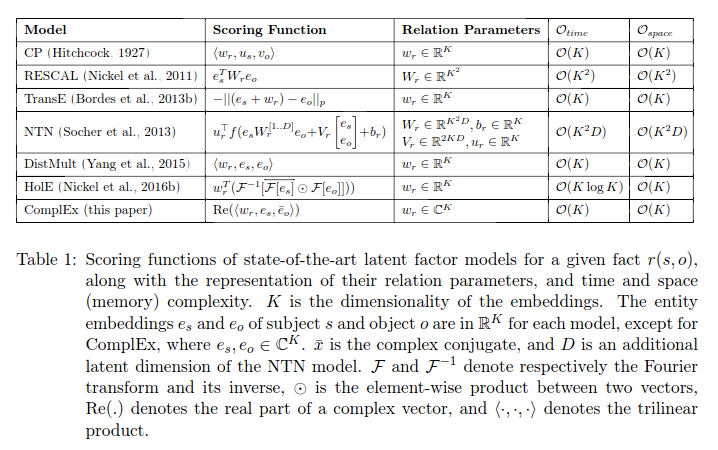
\includegraphics[width=\textwidth,keepaspectratio]{models.png}
\end{figure}

Existing models for knowledge graphs are based on the following compositional operators:

\subsubsection*{Tensor Product} 
Given entity embeddings $\textbf{a}, \textbf{b} \, \epsilon\, \R^d$ , tensor product models represent pairs of entities via $\textbf{a} \,o\,\textbf{b} = \textbf{a} \otimes  \textbf{b} \,\epsilon\,R^{d^2}$ \newline
RESCAL\cite{Nickel_athree-way} is one such compositional models which uses the tensor product. While the tensor product allows to capture rich interactions, its main problem as a compositional operator lies in the fact that it requires a large number of parameters.

\subsubsection{Holographic Embeddings(HoLE)}
Nickel et al.\cite{DBLP:journals/corr/NickelRP15} developed this model. Here the compositional operator used is the  circular correlation of vectors to represent pairs of entities, i.e 
$$ \textbf{a} \,o\, \textbf{b} = \textbf{a} \star \textbf{b} $$
where $ \star : \R^d \,X\, \R^d \rightarrow \R^d $ denotes circular correlation\cite{} :
$$ [\textbf{a} \star \textbf{b}]_k = \sum_{i=0}^{d-1} a_i\, b_{(k+i)mod\,d} $$

As a compositional operator, circular correlation can be
interpreted as a compression of the tensor product.

\phantomsection
\label{neural}
A natural thought that arises is that we can simply use a generic neural network using the embeddings $\textbf{e}_s, \textbf{e}_r$ as input to the network which generate O(d) (let's say 2d) features  instead of the circular correlation which is supposed to work even better.

\subsubsection{ComplEx Embeddings}
The idea of this paper\cite{DBLP:journals/corr/TrouillonWRGB16} was to use two embeddings for a entity instead of one, and they represented those two two embeddings with a complex valued vector. 
\begin{align*}
\eta_{sro} = \phi_r(s, o; \Theta) &= Re(\textbf{e}_s \textbf{W}_r \textbf{e}_o)\\
 &= Re(\sum^{K}_{k=1}w_{rk}e_{sk}\bar{e}_{ok})\\
 &= Re(\langle w_r , e_s, \bar{e}_o  \rangle )
\end{align*}
where $\sigma(\eta_{sro})$ denotes the probability that r(s, o) is true.
Here $Re<\cdot>$ denotes the real part of a imaginary vector. Also,  $e_s, e_o\, \epsilon \, \mathbb{C}_K$
are the rows in E corresponding to the entities s and o; $w_r = diag(W_r) \, \epsilon \, \mathbb{C}_K$ is a complex vector.
\begin{align*}
Re(\langle w_r , e_s, \bar{e}_o  \rangle ) &= \langle Re(w_r), Re(e_s), Re(e_o) \rangle \\
&+ \langle Re(w_r), Im(e_s), Im(e_o) \rangle \\
&+ \langle Im(w_r), Re(e_s), Im(e_o) \rangle \\
&- \langle Im(w_r), Im(e_s), Im(e_o) \rangle \\
\end{align*}

These embeddings can model both symmetric and antisymmetric relations. Although, this model just identifies  another possible way to find interactions between two embeddings. The neural network approach as mentioned \hyperref[neural]{here} is even more generic.

\section{Entity Embeddings}
\label{entity}
Conceptual spaces are geometric representations of conceptual knowledge, in which entities correspond
to points, natural properties correspond to
convex regions, and the dimensions of the space
correspond to salient features. While conceptual
spaces enable elegant models of various cognitive
phenomena, the lack of automated methods for
constructing such representations have so far limited
their application in artificial intelligence.\newline

Jameel et al.\cite{DBLP:conf/coling/JameelS16} proposed a method in which they learnt a vector-space embedding of entities from Wikipedia and constrained this embedding such that entities of the same semantic type are located in
some lower-dimensional subspace using nuclear norm\cite{2007arXiv0706.4138R} regularization.
The model they proposed has the following form:
$$ J = \alpha J_{text} + (1 − \alpha)(J_{type} + J_{rel}) + \beta J_{reg}$$

Component $J_{text}$ will be used to constrain the representation
of the entities based on their textual description,
$J_{type}$ will impose the constraint that entities of the same type
belong to a particular subspace, $J_{rel}$ will use the relations in R to improve the alignment between these subspaces, and $J_{reg}$ is a regularization component which will allow the model to automatically select the most appropriate number of dimensions for every subspace.\\

This model is penalizing loss function $J_{type}$ by a global variable $\alpha$ instead of using different $\alpha$ values for different types.
The authors of this paper\cite{} point out that nuclear
norm regularization allows their model to automatically
select the most appropriate number of dimensions for the subspace
corresponding to each type. So, can we constraint embeddings in bounded regions using this method?  This is one such question which should be investigated experimentally.\\

Bouraoui et al.\cite{DBLP:conf/aaai/BouraouiJS17} proposed a new method for inductive reasoning with ontologies which consisted of using a form of
Bayesian inference over interpretable feature representations
that are obtained from a learned vector space embedding using the method as proposed \hyperref[entity]{above}. Though the idea of this paper was nice, there were a lot of assumptions that seem to be over-simplifying the problem of knowledge base completion.\\

Recently, Yamada et al\cite{DBLP:journals/corr/YamadaS0T16},  proposed a novel embedding method specifically designed for Named Entity Disambiguation. The proposed method jointly maps words and entities into the same continuous vector space. The method extends the skip-gram model by using two models. The KB graph model learns the relatedness of entities using the link structure of the KB, whereas the anchor context model aims to align vectors such that similar words and entities occur close to one another in the vector space by leveraging KB anchors and their context words.

\section{Conclusion}
We discussed a lot of possible extensions for the existing embedding models and raised some questions which are still unanswered. The next logical step is to try out those ideas and find answers to some of the questions we raised!

\bibliographystyle{unsrt}
\addtocounter{section}{1}
\addcontentsline{toc}{section}{Bibliography}
\bibliography{report}

\end{document} to your LaTeX file where you want your
% title page.
%
%%%%%%%%%%%%%%%%%%%%%%%%%%%%%%%%%%%%%%%%%
%\title{Title page with logo}
%----------------------------------------------------------------------------------------
%	PACKAGES AND OTHER DOCUMENT CONFIGURATIONS
%----------------------------------------------------------------------------------------

\documentclass[12pt]{article}
\usepackage[english]{babel}
\usepackage[utf8x]{inputenc}
\usepackage{amsmath}
\usepackage{graphicx}
\usepackage{textcomp}
\usepackage{hyperref}
\usepackage[colorinlistoftodos]{todonotes}
\usepackage{xcolor}
\hypersetup{
    colorlinks,
    linkcolor={blue!50!black},
    citecolor={blue!50!black},
    urlcolor={blue!80!black}
}

\newcommand{\textapprox}{\raisebox{0.5ex}{\texttildelow}}
\newcommand\tab[1][1cm]{\hspace*{#1}}
\begin{document}

\begin{titlepage}

\newcommand{\HRule}{\rule{\linewidth}{0.5mm}} % Defines a new command for the horizontal lines, change thickness here

\center % Center everything on the page
 
%----------------------------------------------------------------------------------------
%	HEADING SECTIONS
%----------------------------------------------------------------------------------------

\textsc{\LARGE Indian Institute of Technology Bombay}\\[1cm] % Name of your university/college
\textsc{\Large Department of Computer Science \& Engineering}\\[0.5cm] % Major heading such as course name
\textsc{\large Seminar Report}\\[0.5cm] % Minor heading such as course title

%----------------------------------------------------------------------------------------
%	TITLE SECTION
%----------------------------------------------------------------------------------------

\HRule \\[0.4cm]
{ \huge \bfseries Adapting Deep Learning Models}\\[0.4cm] % Title of your document
\HRule \\[1.5cm]
 
%----------------------------------------------------------------------------------------
%	AUTHOR SECTION
%----------------------------------------------------------------------------------------

\begin{minipage}{0.4\textwidth}
\begin{flushleft} \large
\emph{Author:}\\
Rishabh \textsc{Agarwal} % Your name
\end{flushleft}
\end{minipage}
~
\begin{minipage}{0.4\textwidth}
\begin{flushright} \large
\emph{Supervisor:} \\
Prof. Sunita \textsc{Sarawagi} % Supervisor's Name
\end{flushright}
\end{minipage}\\[2cm]

% If you don't want a supervisor, uncomment the two lines below and remove the section above
%\Large \emph{Author:}\\
%John \textsc{Smith}\\[3cm] % Your name

%----------------------------------------------------------------------------------------
%	DATE SECTION
%----------------------------------------------------------------------------------------

{\large \today}\\[2cm] % Date, change the \today to a set date if you want to be precise

%----------------------------------------------------------------------------------------
%	LOGO SECTION
%----------------------------------------------------------------------------------------


\includegraphics[height=4cm]{logo.jpg}\\[1cm] % Include a department/university logo - this will require the graphicx package
 
%----------------------------------------------------------------------------------------

\vfill % Fill the rest of the page with whitespace

\end{titlepage}


\tableofcontents
\pagebreak

\begin{abstract}
Learning quickly is a hallmark of human intelligence, whether it involves recognizing objects from a few examples or quickly learning new skills after just minutes of experience. One of the current limitations of deep learning is the need for tremendous amounts of data.
Finding techniques to achieve state-of-the-art performance on tasks with orders of magnitude less data is a very active research area. In this work, we survey some of the recent approaches to tackle this problem of learning new concepts rapidly with very little data.
\end{abstract}

\section{Introduction}

We need for massive amounts of data to train deep neural networks. In contrast, humans require comparatively little data to learn a new behavior or to rapidly shift away from an old behavior. For example,  a child can generalize the concept of “giraffe” from a single picture in a book, yet our best deep learning systems need hundreds or thousands of examples.\\

It is estimated that a child has learned almost all of the $10\sim30$ thousand object categories in the world by the age of six. This is due not only to the human mind's computational power, but also to its ability to synthesize and learn new object classes from existing information about different, previously learned classes.\\

Our artificial agents should be able to do the same, learning and adapting quickly from only a few examples, and continuing to adapt as more data becomes available. This kind of fast and flexible learning is challenging, since the agent must integrate its prior experience with a small amount of new information, while avoiding overfitting to the new data. Furthermore, the form of prior experience and new data will depend on the task.

\section{Problem Statement}
The problem which we'd discuss in this work is as follows:\newline
We are given a large global dataset and a small amount of “personal" labeled data.
We trained a model (mostly a deep neural network) using the global data. The goal is to adapt this model for the limited labeled data so as to personalize the trained model. 
This problem has various applications in speech recognition, hand writing recognition, and text conversation bots.\\

Suppose we want to build an app to recognize the handwriting of a person. Assume we are given access to a large global dataset of handwritten characters such as MNIST\cite{lecun-mnisthandwrittendigit-2010}. Using this dataset, we trained a DNN model and deployed this model in our app. But this app would not work well for all the users as each user have a unique handwriting which may be significantly differ from the  handwritings the model have seen in the global dataset. Therefore, we need to adapt our model for each user utilizing the few samples ( $1\sim10$ ) we obtain from them.

\section{How to solve the problem?}
Since we want to incorporate our prior experience in solving the adaptation problem, the area of \textbf{Transfer Learning and Domain Adaptation} are quite relevant to it.\\ 

According to {Goodfellow et al.}\cite{Goodfellow-et-al-2016} Transfer Learning and Domain Adaptation refer to "the situation where what has been learned in one setting (i.e., distribution P1) is exploited to improve generalization in another setting (say distribution P2)". These fields are described in detail in the sections~\ref{sec:transfer} and~\ref{sec:domain}.\\

This problem can also be posed as a \textbf{few-shot learning} problem and is discussed  further in section~\ref{sec:few-shot}.

\subsection{Transfer Learning}
\label{sec:transfer}
In transfer learning, we first train a base network on a base dataset and task, and then we repurpose the learned features, or transfer them, to a second target network to be trained on a target dataset and task. \\

The usual approach is to train a base network and then copy its first \textbf{N} layers to the first n layers of a target network.Currently, no basis is provided for picking a particular layer from the pretrained network when using transfer learning.\\ 

Therefore, it's natural to think about this question: \textbf{How much effective is Transfer Learning?} What value of \textbf{N} should be used? Do we fine-tune the transferred network to the new task, or are they left frozen? \\

    {Yosinski et al.}\cite{DBLP:journals/corr/YosinskiCBL14}, sheds some light on this issue and tries to experimentally quantify the generality versus specificity of neurons in each layer of a deep CNN when used for transfer learning tasks. I have discussed their experimental setup and the results below.
    \subparagraph{Experiment Setup \& Results} Experiments were performed by training two \textbf{M}-layered neural nets (here n = 8) (call them A \& B) on two disjoint datasets obtained from ImageNet.\\
    
    Then, transfer learning was performed by picking first K layers of one of the networks (let's say A) and using them with last N-K layers of either A or B both with and without fine-tuning. \\

From these experiments, some of the non-obvious conclusions are:
      \begin{itemize}
       \item There are 2 separate issues that cause performance degradation when using
    transferred features without fine-tuning:\\ 
    (i) the specificity of the features themselves, and\\
    (ii) optimization difficulties due to splitting the base network between co-adapted neurons on neighboring layers.
        \item Initializing a network with transferred features from almost any number of layers can produce a boost to generalization performance after fine-tuning to a new dataset.
      \end{itemize}
Though, the above results, should be taken with a pinch of salt, as they are heavily dependent on the optimization algorithm used (here, SGD+Momentum) and the transfer task. But the take-away from this paper was that \textbf{transfer learning always helps if there is some similarity between the two tasks}.

\subsection{Domain Adaptation}
\label{sec:domain}
Adaptation of neural network models in the context of speech, \textbf{speaker adaptation}, is well researched.  Acoustic models have evolved starting from GMM\cite{wiki:GMM} or HMM models to hybrid models that are NN/{HMM}\cite{wiki:HMM}, deep neural networks to LSTM\cite{olah} based RNN models.\\

The problem of low performance due to train and test domain differences is acute in speech and is well addressed in the past even before the introduction of neural networks.\\

We shall further discuss the domain adaptation problem only in the context of neural networks.

\subsubsection{Speaker Adaptation of hybrid NN/HMM based on speaker codes}
In this work\cite{6639211}, a fast speaker adaptation method was proposed for the hybrid NN-HMM speech recognition model. In a NN/HMM model, the GMM component that is used to estimate the emission probabilities of each state is replaced by neural network which when fed with the features vector outputs the posterior over HMM state labels.\\

\begin{figure}
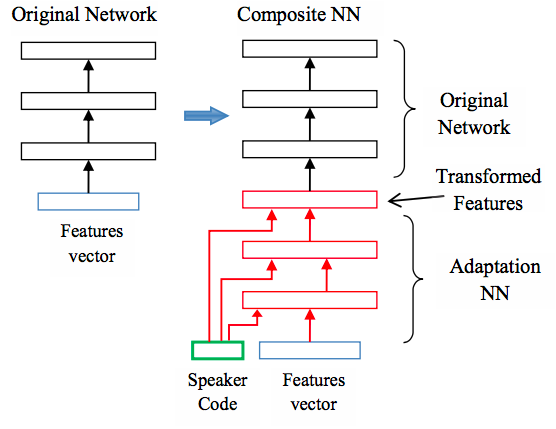
\includegraphics[height=8cm, width=\textwidth,keepaspectratio]{speaker.png}
\caption{\label{fig:speaker}{Speaker adaptation of the hybrid NN-HMM model based on speaker code}}
\end{figure}

As shown in figure~\ref{fig:speaker}, the proposed adaptation method relies on learning adaptation NN and speaker codes. All weights of adaptation NN are standard fully connected layers. The transformed feature vector should have the same dimension as the input feature vector. During the adaptation phase, both the weights of adaptation NN and speaker need to be learned.

\subsubsection{Using I-Vector inputs to improve speaker independence}

This paper\cite{42536} proposed providing additional utterance-level features as inputs to a DNN to facilitate speaker, channel and background normalization.
\subparagraph{i-Vectors or identity vectors} According to the authors "i-vectors encode precisely those effects to which we want our ASR system to be invariant: speaker, channel and background noise." These vectors are generally used in speaker recognition and verification.\\

\begin{figure}
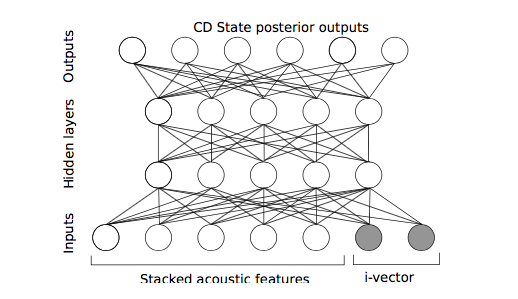
\includegraphics[width=\textwidth]{i-vectors.png}
\caption{\label{fig:i-vectors}{Diagram of a 2-hidden layer neural network with inputs augmented with i-vectors}}
\end{figure}

As shown in the figure~\ref{fig:i-vectors}, the idea is to provide the input with characterization of the speaker should enable it to normalize the signal with respect to them and thus better able to make its outputs invariant to them.

\subsection{Few-Shot Learning}
\label{sec:few-shot}

One obvious approach to this problem is to use transfer learning as described in Section ~\ref{sec:transfer} above. But since only have few examples, the normal approach to transfer learning doesn't work.\\
This can be mitigated by viewing it as a few-shot learning problem, an extreme case of transfer learning, which involves learning a new class with only few labeled examples. In this formulation, the limited personal data acts as the new examples on which we apply few-shot learning. This.\
There are two major approaches for this formulation of the problem which are quite different from the speaker adaptation approaches discussed above in section~\ref{sec:domain}\:
\begin{itemize}
\setlength\itemsep{0.1em}
\item Meta Learning or ``Learning to learn"
\item Memory Augmented Neural Networks
\end{itemize}

\subsection{Meta Learning}

According to {Santaro et al.}\cite{DBLP:journals/corr/SantoroBBWL16}, meta-learning generally refers to a scenario in which an agent learns at two levels, each associated with different time scales. Rapid learning occurs within a task, for example, when learning to accurately classify within a particular dataset. This learning is guided by knowledge
accrued more gradually across tasks, which captures the way in which task structure varies across target domains.

\subsubsection{Meta-Learning Problem Set-Up}
\begin{itemize}
\setlength\itemsep{0.1em}
  \item Consider a model, denoted \textbf{M} , that maps observations \textbf{x} to outputs \textbf{a}
  \item \textbf{M} is trained to be able to adapt to a large or infinite number of tasks
  \item Each task  \textbf{\textit{T}} = $ \{L(x_1 , a_1, \ldots , x_H , a_H ), q(x_1), q(x_{t+1}|x_t , a_t ), H\} $ where\\ 
           \tab \textbf{L, H} are the loss function and episode length resp,\\          
           \tab $ q(x_1) $ is the initial distribution over examples,\\
           \tab $ q(x_{t+1}|x_t , a_t) $ is the transition distribution\\      
  \item Define $\rho$(\textit{T}) to be a distribution over tasks
\end{itemize}
In the case of i.i.d. supervised learning problems, the length is H = 1.\newline
During meta-training, 
\begin{itemize}
\setlength\itemsep{0.1em}
  \item A task $\textit{T}_i$ is sampled from $\rho$(\textit{T})
  \item In the K-shot learning setting, \textbf{M} is trained with \textit{K} samples and feedback from the corresponding loss $L_{T_i}$ from $\textit{T}_i$
  \item \textbf{M} is then tested on new samples from $\textit{T}_i$ 
  \item The model \textbf{M} is then improved by considering how
the test error on new data from $q_i$ changes with respect to
the parameters.
\end{itemize}
In effect, the test error on sampled tasks $T_i$ serves as the training error of the meta-learning process.\newline
During meta-testing:
\begin{itemize}
\setlength\itemsep{0.1em}
\item New tasks (held out during meta-training) are sampled from $\rho$(\textit{T})
\item Meta-performance is measured by the model's performance after learning from K samples. Generally, tasks used for meta-testing are held out during meta-training
\end{itemize}

\subsubsection{Matching Networks for One Shot Learning} 
This is a paper\cite{DBLP:journals/corr/SantoroBBWL16} on one-shot learning, where we try to learn a class based on very few (or indeed, 1) training examples. The Matching Nets architecture described in this paper \textbf{blends deep learning with nearest neighbour, using neural networks augmented with memory (LSTMs)!}\\ 

\begin{figure}
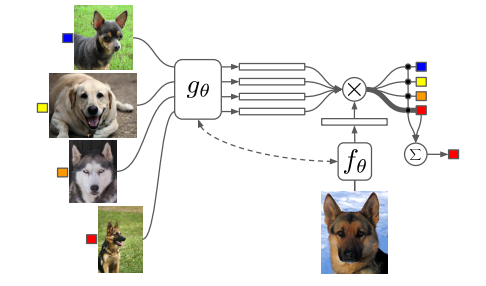
\includegraphics[width=\textwidth]{matching_network.png}
\caption{\label{fig:MATCHING_NETS}{Matching Nets Architecture.}}
\end{figure}

\begin{itemize}
\item \textbf{The Training Protocol}\\
As the authors point out in the conclusion ``one-shot learning is much easier if you train the network to do one-shot learning". Therefore, we want the test-time protocol to exactly match the training time protocol.
To create each``episode" of training from a dataset of examples then:
\begin{itemize}
\item  Sample a task T from the training data, e.g. select 5 labels, and up to 5 examples per label (i.e. 5-25 examples).
\item To form one episode sample a label set L (e.g. {cats, dogs}) and then use L to sample the support set S and a batch B of examples to evaluate loss on.
\item  The Matching Net is then trained to minimize the error predicting the labels in the batch B conditioned on the support set S. 
\end{itemize}
This is a form of meta-learning since the training procedure explicitly learns to learn from a given support set to minimize a loss over a batch.

\item \textbf{The model}\\
Basically we're building a differentiable nearest neighbor++. The output $\hat{y}$ for a test example $\hat{x}$ is computed very similar to what you might see in Nearest Neighbors: 
$$\hat{y} = \sum_{i=1}^{n} a(x, x_i)y_i$$

where \textbf{a} acts as a kernel, computing the extent to which $\hat{x}$ is similar to a training example $x_i$, and then the labels from the training examples $y_i$ are weight-blended together accordingly. The paper doesn't mention this but I assume for classification $y_i$ would presumably be one-hot vectors.

Now, we're going to embed both the training examples $x_i$ and the test example $\hat{x}$, and we'll interpret their inner products (or here a cosine similarity) as the ``match", and pass that through a softmax to get normalized mixing weights so they add up to 1.

$$ a(x,x_i) = e^{c(f(\hat{x}), g(x_i))}/ \sum_{i=1}^{n} e^{c(f(\hat{x}), g(x_i))} $$

Here \textbf{c()} is cosine distance, which is implemented by normalizing the two input vectors to have unit L2 norm and taking a dot product. \textbf{$f(\hat{x})$} corresponds to the embedding of a test example and the function \textbf{$g(x_i)$} is the training embedding of the $i^{th}$ training example.\newline

\textbf{Embedding the training examples.} The function g is a bidirectional LSTM over the examples:

$$ \overrightarrow{h}_i, \overrightarrow{c}_i = LSTM(g'(x_i),\overrightarrow{h}_{i-1},\overrightarrow{c}_{i-1})$$
$$\overleftarrow{h}_i, \overleftarrow{c}_i = LSTM(g'(x_i),\overleftarrow{h}_{i-1},\overleftarrow{c}_{i-1})$$

i.e. encoding of $i^{th}$ example $x_i$ is a function of its``raw" embedding $g'(x_i)$ and the embedding of its friends, communicated through the bidirectional network's hidden states i.e. each training example is a function of not just itself but all of its friends in the set. This is part of the ++ above, because in a normal nearest neighbor you wouldn't change the representation of an example as a function of the other data points in the training set.\\

\textbf{Embedding the test example}
The function f is an LSTM that processes for a fixed amount (K time steps) and at each point also attends over the examples in the training set. The encoding is the last hidden state of the LSTM. Again, this way we're allowing the network to change its encoding of the test example as a function of the training examples.

$$\hat{h}_k, c_k = LSTM(f'(\hat{x},[h_{k-1},r_{k-1}], c_{k-1})$$
$$h_k = \hat{h}_k + f'(\hat(x)$$
$$r_{k-1} = \sum_{i=1}^{|S|} a(h_{k-1}, g(x_i))g(x_i)$$
$$ a(h_{k-1}, g(x_i))= softmax(h^T_{k-1}g(x_i))$$

It's really just a vanilla LSTM with attention where the input at each time step is constant $(f'(\hat{x})$, an encoding of the test example all by itself) and the hidden state is a function of previous hidden state but also a concatenated readout vector r, which we obtain by attending over the encoded training examples (encoded with g from above).\\

Experiments were done on the Omniglot dataset, ImageNet and they also introduced an one-shot task on the Penn Treebank.

\end{itemize}

\subsubsection{MAML for Fast Adaptation of Deep Networks} 
The novel idea of this paper\cite{1703.03400} is to \textbf{train the model's initial parameters such that it has maximal performance on a new task after the parameters have been updated}. This can be viewed as building an internal representation that is broadly suitable for many tasks.\\

This method assumes that the model will be fine-tuned using a gradient-based learning rule on a new task and therefore,  tries to learn a model such that this gradient-based learning rule can make rapid progress on new tasks drawn from $\rho$(\textit{T}), without overfitting.
\subparagraph{MAML Algorithm}
Consider a model represented by a parametrized function $\mathbf{M_\theta}$ with parameters $\theta$. When adapting to a new task $\textit{T}_i$, the model's parameters $\theta$ becomes ${\theta_i}^\prime$. Train the model parameters by optimizing for the performance of $\mathbf{M_{{\theta_i}^\prime}}$ w.r.t $\theta$ across tasks sampled from $\rho$(\textit{T}). Please refer to Figure~\ref{fig:MAML} and ~\ref{fig:MAML} for the generic and supervised learning specific algorithm respectively.\\

\begin{figure}
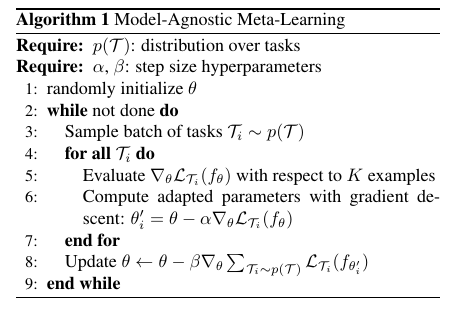
\includegraphics[height=8cm,width=\textwidth,keepaspectratio]{maml_1.png}
\caption{\label{fig:MAML}The generic MAML algorithm}
\end{figure}

\begin{figure}
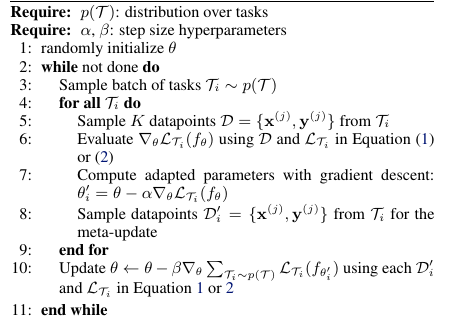
\includegraphics[height=8.5cm,width=\textwidth,keepaspectratio]{maml_2.png}
\caption{\label{fig:MAML2}MAML for few-shot supervised learning}
\end{figure}

This model has the advantage of being agnostic to the form of the model \textbf{M} and to the particular learning task. Also, it does not introduce any additional parameters into the learning process. In addition to above, it produces a good weight initialization, and thus, further adaptation can be performed with any amount of data and any number of gradient steps.\\

The only limitation of this paper is that meta-learning training phase can underfit because of small number of adaptation steps. Also, an additional hyperparameter, which is the model's step size $\alpha$ is introduced, which was obtained though fine tuning.

\subsection{Memory Augmented Neural Networks}

\subsubsection{Learning to Remember Rare Events}

% \subsection{Comments}

% Comments can be added to the margins of the document using the \todo{Here's a comment in the margin!} todo command, as shown in the example on the right. You can also add inline comments too:

% \todo[inline, color=green!40]{This is an inline comment.}

% \subsection{Tables and Figures}

% Use the table and tabular commands for basic tables --- see Table~\ref{tab:widgets}, for example. You can upload a figure (JPEG, PNG or PDF) using the files menu. To include it in your document, use the includegraphics command as in the code for Figure~\ref{fig:frog} below.

% % Commands to include a figure:
% \begin{figure}
% \centering
% 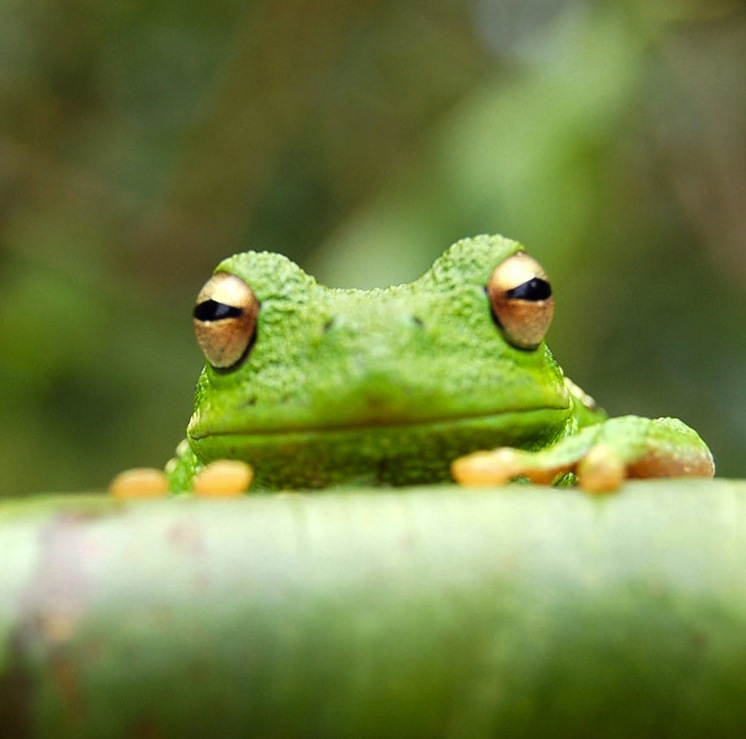
\includegraphics[width=0.5\textwidth]{frog.jpg}
% \caption{\label{fig:frog}This is a figure caption.}
% \end{figure}

% % \begin{table}
% % \centering
% % \begin{tabular}{l|r}
% % Item & Quantity \\\hline
% % Widgets & 42 \\
% % Gadgets & 13
% % \end{tabular}
% % \caption{\label{tab:widgets}An example table.}
% % \end{table}

% \subsection{Mathematics}

% \LaTeX{} is great at typesetting mathematics. Let $X_1, X_2, \ldots, X_n$ be a sequence of independent and identically distributed random variables with $\text{E}[X_i] = \mu$ and $\text{Var}[X_i] = \sigma^2 < \infty$, and let
% $$S_n = \frac{X_1 + X_2 + \cdots + X_n}{n}
%       = \frac{1}{n}\sum_{i}^{n} X_i$$
% denote their mean. Then as $n$ approaches infinity, the random variables $\sqrt{n}(S_n - \mu)$ converge in distribution to a normal $\mathcal{N}(0, \sigma^2)$.

% \subsection{Lists}

% You can make lists with automatic numbering \dots

% \begin{enumerate}
% \item Like this,
% \item and like this.
% \end{enumerate}
% \dots or bullet points \dots
% \begin{itemize}
% \item Like this,
% \item and like this.
% \end{itemize}

% We hope you find write\LaTeX\ useful, and please let us know if you have any feedback using the help menu above.

\bibliographystyle{unsrt}
\addtocounter{section}{1}
\addcontentsline{toc}{section}{Bibliography}
\bibliography{report}

\end{document}